\documentclass[12pt]{article}
\usepackage[sectionbib]{natbib}
\usepackage{array,epsfig,fancyheadings,rotating}
\usepackage[hidelinks]{hyperref}
\usepackage{sectsty, secdot}
\sectionfont{\fontsize{12}{14pt plus.8pt minus .6pt}\selectfont}
\renewcommand{\theequation}{\thesection\arabic{equation}}
\subsectionfont{\fontsize{12}{14pt plus.8pt minus .6pt}\selectfont}

\textwidth=31.9pc
\textheight=46.5pc
\oddsidemargin=1pc
\evensidemargin=1pc
\headsep=15pt
\topmargin=.6cm
\parindent=1.7pc
\parskip=0pt

\usepackage{amsmath}
\usepackage{amssymb}
\usepackage{amsfonts}
\usepackage{multirow}
\usepackage{amsthm}
\usepackage{graphicx}
\usepackage{booktabs}
\usepackage{xr}
\externaldocument[S-]{supplement}

\setcounter{page}{1}
\newtheorem{theorem}{Theorem}
\newtheorem{lemma}{Lemma}
\newtheorem{corollary}{Corollary}
\newtheorem{proposition}{Proposition}
\theoremstyle{definition}
\newtheorem{definition}{Definition}
\newtheorem{example}{Example}
\newtheorem{remark}{Remark}
\pagestyle{fancy}

\newcommand{\pr}{\mathrm{pr}}
\newcommand{\LC}{\mathcal{L}}
\newcommand{\B}{\mathcal{B}}
\newcommand{\E}{\mathcal{E}}
\newcommand{\var}{\mathrm{var}}
\newcommand{\Bin}{\mathrm{Bin}}

\def\n{\noindent}
\lhead[\fancyplain{} \leftmark]{}
\chead[]{}
\rhead[]{\fancyplain{}\rightmark}
\cfoot{}

\begin{document}

\renewcommand{\baselinestretch}{2}

\markright{ \hbox{\footnotesize\rm Statistica Sinica}\hfill\\[-13pt]
\hbox{\footnotesize\rm}\hfill }

\markboth{\hfill{\footnotesize\rm KUN WOO PARK} \hfill}
{\hfill {\footnotesize\rm LATENT COVERAGE FROM NOISY CALIBRATION} \hfill}

\renewcommand{\thefootnote}{}
$\ $\par

\fontsize{12}{14pt plus.8pt minus .6pt}\selectfont \vspace{0.8pc}
\centerline{\large\bf LATENT COVERAGE FROM NOISY CALIBRATION}
\vspace{.4cm}
\centerline{Kun Woo Park}
\vspace{.4cm}
\centerline{\it Kookmin University}
\vspace{.55cm} \fontsize{9}{11.5pt plus.8pt minus.6pt}\selectfont

\begin{quotation}
\noindent {\it Abstract:}
Prediction intervals for a latent quantity, such as the true mean of an unsampled small area or a response measured with error, are often calibrated on noisy proxies. We ask what latent coverage a threshold calibrated on noisy scores guarantees when the law and the variance of the noise are unknown and may differ between units, and what is the smallest correction that keeps the guarantee. The answer turns on the shape of the latent law. Unimodality, even with mean zero, gains nothing over no shape assumption: with median-zero noise, noisy coverage of ninety percent guarantees only eighty percent. Bi-log-concavity, which allows asymmetry and some multimodality, recovers almost all of the loss. We give the required noisy level exactly for Gaussian and symmetric unimodal noise, including a new closed form for Gaussian noise, and within certified bounds for mean-zero log-concave noise. These levels define a conformal rank that needs no noise variances, keeps the latent guarantee with prescribed probability, and cannot be lowered, whereas the usual high-probability rank loses the guarantee as the calibration sample grows. The guarantee extends to latent laws that differ between units, under an ordering condition that cannot be dropped. In simulations the rank cost at most three percent of width over the usual rank, and was no wider than LatentCP, which is given the noise variances; in a school-district application it needed no variance estimates.

\vspace{9pt}
\noindent {\it Key words and phrases:}
Bi-log-concavity, conformal prediction, measurement error, small area estimation, tolerance interval.
\par
\end{quotation}\par

\def\thefigure{\arabic{figure}}
\def\thetable{\arabic{table}}
\renewcommand{\theequation}{\thesection.\arabic{equation}}

\fontsize{12}{14pt plus.8pt minus .6pt}\selectfont

%=============================================================================================
\section{Introduction}\label{sec:intro}

Suppose that a residual $W$, the latent target minus a centre fitted on independent training data, is observed only through $V = W + e$, with noise $e$ independent of $W$. A survey statistician who calibrates a prediction interval for the true mean of an unsampled area on the direct estimates of sampled areas is in this position \citep{fay1979}, as is a conformal analyst whose calibration responses carry measurement error \citep{einbinder2024, cohen2025}. The threshold $t$ at which the noisy scores $|V|$ have coverage $p$ is observable. The quantity of interest is the latent coverage $\pr(|W| \le t)$. In both examples the noise law and its variance are often unknown, or known only through rough estimates, and they differ from unit to unit: direct estimates of areas with different sample sizes have different variances, and measurement devices differ.

This paper asks two questions. First, what latent coverage does noisy coverage $p$ guarantee, uniformly over a class of latent laws and over noise laws of every scale? Second, when the noise laws and scales are unknown and differ between units, which conformal rank keeps a latent guarantee with prescribed probability, and what is the smallest such rank?

Two answers to the first question are known. If $W$ and $e$ are both symmetric and unimodal, the theorem of \citet{anderson1955} gives $\pr(|W + e| \le t) \le \pr(|W| \le t)$, so the noisy threshold is conservative \citep{einbinder2024}. Without a shape assumption, median-zero noise turns a noisy level $1 - \alpha$ into a latent level $1 - 2\alpha$ \citep[Proposition~2.3]{guille2024}. Symmetry of the latent residual is a strong assumption: residuals of area means of skewed outcomes are asymmetric, and a population of two types of areas gives a bimodal residual. The shape-free answer is very costly: at $\alpha = 0.1$ it halves the allowed failure.

We take the latent law to be bi-log-concave \citep{dumbgen2017}: its distribution function $F$ is continuous and both $\log F$ and $\log(1 - F)$ are concave. The class contains the log-concave laws and some multimodal ones, and does not require symmetry. Our contributions are as follows.
\begin{enumerate}
\item \emph{A boundary.} Unimodality of the latent law, even with mean zero, gives nothing over no shape assumption (Proposition~\ref{prop:latentshape}); bi-log-concavity recovers almost all of the loss.
\item \emph{Exact levels.} For each class of noise laws we characterize the noisy level that guarantees latent coverage $q$ (Proposition~\ref{prop:general}, Theorem~\ref{thm:classes}). It is exact for symmetric unimodal noise, and, by a new closed form, for Gaussian noise (Theorem~\ref{thm:gauss}); for mean-zero log-concave noise it lies within certified bounds. In both exact cases the transfer is nontrivial exactly when $q > \mathrm{e}^{-1}$.
\item \emph{A rank that needs no variances and cannot be lowered.} These levels give a conformal rank that keeps the latent guarantee with probability at least $1 - \delta$ when the noise laws and scales are unknown and differ between units (Theorem~\ref{thm:rank}). At an extremal law its latent reliability tends to exactly $1 - \delta$, so no smaller rank is valid, whereas the usual high-probability rank loses the guarantee as the calibration sample grows (Proposition~\ref{prop:fail}). The guarantee extends to latent laws that differ between units under a quantile ordering condition, which cannot simply be dropped (Corollary~\ref{cor:hetero}).
\item \emph{Evidence in three roles.} Exact reliability computations show when the correction is needed (\S~\ref{sec:need}); simulations with the same information and against existing methods show what it costs (\S\S~\ref{sec:cost}--\ref{sec:competitors}); a school-district application shows how it behaves on data (\S~\ref{sec:application}).
\end{enumerate}

Related methods target different quantities or use more information; Table~\ref{tab:methods} places them by both. LatentCP \citep{zheng2026} inverts a conformal set for the response through a known forward model and gives a marginal latent guarantee. \citet{cohen2025} estimate the noise-free conformal threshold under Gaussian label noise of known variance, without a finite-sample latent guarantee. Conformal intervals for small areas cover observable responses \citep{bersson2024} or the expectations of sampled units conditional on the sample \citep{zhang2026}. Empirical Bayes and parametric small-area intervals \citep{armstrong2022, ignatiadis2022, hallmaiti2006, yoshimori2014} concern sampled units or rely on a model for the latent effects; the Fay--Herriot interval with a bootstrap tolerance multiplier is valid under the normal model. None of these addresses a guarantee over a nonparametric class of latent laws when the noise law and variance are unknown.

\begin{table}[htbp]
\renewcommand{\baselinestretch}{1}
\caption{Interval methods for a latent target calibrated on noisy scores, by the noise information used and the guarantee targeted}
\label{tab:methods}
\centering
\fontsize{9}{11pt}\selectfont
\begin{tabular}{p{4.1cm}p{3.6cm}p{4.3cm}}
\toprule
method & noise information & guarantee \\
\midrule
noisy threshold, usual rank & none & none for the latent target \\
Anderson's theorem \citep{einbinder2024} & symmetric unimodal noise & latent, symmetric unimodal latent law \\
shape-free level \citep{guille2024} & median-zero noise & latent, any latent law \\
LatentCP \citep{zheng2026} & known forward model & marginal latent \\
deconvolution threshold \citep{cohen2025} & known Gaussian noise variances & none in finite samples \\
Fay--Herriot tolerance interval & known variances, normal model & under the model \\
this paper, Theorem~\ref{thm:rank} & a class of noise laws only & latent with probability $1 - \delta$, bi-log-concave latent law \\
\bottomrule
\end{tabular}
\end{table}

Section~\ref{sec:setting} sets up the problem. Section~\ref{sec:transfer} gives the coverage transfer and Section~\ref{sec:procedure} the calibration rank. Section~\ref{sec:known} shows what a known Gaussian noise variance adds. Sections~\ref{sec:numerical} and~\ref{sec:application} give the numerical evidence and the application, and Section~\ref{sec:discussion} discusses limitations and open problems. Proofs, certificates and further results are in the Supplementary Material.

%=============================================================================================
\section{Setting}\label{sec:setting}

Let $\LC$ be the class of log-concave laws on the real line, including point masses, and $\B \supset \LC$ the class of laws that are point masses or have a continuous distribution function $F$ with $\log F$ and $\log(1 - F)$ concave. Both classes are closed under translation and scaling, and convolution with a log-concave law preserves them, by the theorem of \citet{prekopa1973} (Supplementary \S~\ref{S-sec:s-prelim}). Bi-log-concave laws have a density except possibly at an atom, and concavity of $\log F$ makes $f/F$ nonincreasing; a mixture of two well separated normal laws with suitable weights is bimodal and still in $\B$ (Supplementary Lemma~\ref{S-lem:bimodal}).

A class $\E$ of noise laws is closed under scaling and negation. The classes considered are Gaussian laws; symmetric unimodal laws; mean-zero log-concave laws; and mean-zero unimodal laws. For a noise law in $\E$ and a latent law, the noisy coverage of $[-t, t]$ is $\pr(|W + e| \le t)$ and the latent coverage is $\pr(|W| \le t)$.

In calibration, $W_1, \ldots, W_K, W_{\rm new}$ are independent latent residuals and $e_i = \sigma_i\epsilon_i$ are independent noises, independent of the residuals, with laws of $\epsilon_i$ in $\E$ that may differ between units and unknown scales $\sigma_i > 0$. The scores $V_i = W_i + e_i$ are independent but not identically distributed. Let $\mathcal D$ denote the calibration data and $T = |V|_{(k)}$, the $k$th smallest of $|V_1|, \ldots, |V_K|$. The interval $[-T, T]$ is placed around the fitted centre of a new unit. We call
\[
\pr_{\mathcal D}\{\pr(|W_{\rm new}| \le T \mid \mathcal D) \ge q\}
\]
the latent reliability of rank $k$: the probability, over calibration samples, that the interval attains latent coverage $q$. A rank is valid at level $1 - \delta$ if its latent reliability is at least $1 - \delta$ for every latent law and every noise configuration in the model. Throughout, $Q_q$ denotes the lower $q$-quantile, $\Phi$ and $\phi$ the standard normal distribution function and density.

%=============================================================================================
\section{Coverage transfer}\label{sec:transfer}

\subsection{One end of the interval}

For a class $\E$ let
\begin{equation}\label{eq:psi}
\Psi_{\E}(q) = \sup_{\epsilon \in \E} E\{\min(1, q \mathrm{e}^{-\epsilon})\}.
\end{equation}
The extremal latent laws are exponential tails, because concavity of $\log F_Y$ limits how fast mass can accumulate below a quantile: with $E_u$ exponential with rate $u > 0$, the law of $b - E_u$ has distribution function $\min\{1, \mathrm{e}^{u(y - b)}\}$.

\begin{proposition}\label{prop:general}
Let $\epsilon$ have a law in $\E$ and be independent of $Y$, with $\log F_Y$ concave. If $\pr(Y + \epsilon \le 0) \ge p > \Psi_{\E}(q)$, then $F_Y(0) \ge q$. If $p < \Psi_{\E}(q)$, some exponential tail $Y$ with $F_Y(0) < q$ and some $\epsilon$ with law in $\E$ have $\pr(Y + \epsilon \le 0) > p$.
\end{proposition}

\begin{proof}
Suppose that $v = F_Y^{-1}(q) > 0$, let $a = \log(1/q)$ and let $u$ be a supergradient of $\log F_Y$ at $v$. Then $F_Y(y) \le \min\{1, q\mathrm{e}^{u(y - v)}\}$, so the exponential tail $v + a/u - E_u$ lies stochastically below $Y$. Adding $\epsilon$ preserves this, and as $v > 0$ and $u\epsilon$ has a law in $\E$,
\[
p \le \pr(Y + \epsilon \le 0) \le \pr(a/u - E_u + \epsilon \le 0) = E\{\min(1, q \mathrm{e}^{-u\epsilon})\} \le \Psi_{\E}(q).
\]
If $\log F_Y$ has no finite supergradient at $v$, as when $Y$ has an atom at $v$ and no mass below it, then $p \le \pr(\epsilon < 0) \le \lim_{u\to\infty} E\{\min(1, q \mathrm{e}^{-u\epsilon})\} \le \Psi_{\E}(q)$. Conversely, $a - E_1$ with noise $\epsilon$ attains $E\{\min(1, q \mathrm{e}^{-\epsilon})\}$; shift it slightly to the right.
\end{proof}

Applied to $Y = (W - t)/s$ for any scale $s > 0$, Proposition~\ref{prop:general} controls the right end of $[-t, t]$; applied to $-W$, which uses concavity of $\log(1 - F_W)$, it controls the left end. For a one-sided interval $(-\infty, t]$ it is the complete answer: noisy coverage above $\Psi_{\E}(q)$ gives latent coverage $q$ whenever $\log F_W$ is concave, and no lower level suffices.

\subsection{Both ends}

A noisy failure probability $1 - p$ may be split in any way between the two ends, and each end transfers separately. Let $\lambda_{\E}(p) = \sup\{q' : \Psi_{\E}(q') < p\}$, the inverse of $\Psi_{\E}$ when $\Psi_{\E}$ is continuous and increasing, and $\phi_{\E}(a) = 1 - \lambda_{\E}(1 - a)$. With $\beta_{\E} = \inf_{\epsilon \in \E} \pr(\epsilon \ge 0)$, $\Psi_{\E}(q') \le 1 - (1 - q')\beta_{\E}$; we assume $\beta_{\E} > 0$, so that $\phi_{\E}(0) = 0$. In words, $\phi_{\E}(a)$ is the largest latent failure probability at one end that is compatible with noisy failure probability $a$ there. With $a_L = \pr(W + e < -t)$ and $a_R = \pr(W + e > t)$, define the sufficient noisy level
\begin{equation}\label{eq:pE}
p_{\E}(q) = \inf\{p : \phi_{\E}(a_L) + \phi_{\E}(a_R) \le 1 - q \text{ whenever } a_L + a_R \le 1 - p\}.
\end{equation}
Noisy coverage above $p_{\E}(q)$ at threshold $t$ gives latent coverage $q$ for every $W \in \B$ and every noise with law in $\E$. Putting all the failure at one end, with small noise so that the other end is untouched, shows that no noisy level below $\Psi_{\E}(q)$ suffices (Supplementary \S~\ref{S-sec:s-oneend}), so $\Psi_{\E}(q) \le p_{\E}(q)$. If $\phi_{\E}$ is convex, then, as $\phi_{\E}(0) = 0$, $\phi_{\E}(a_L) + \phi_{\E}(a_R) \le \phi_{\E}(a_L + a_R)$: the worst split puts the whole failure at one end, and $p_{\E}(q) = \Psi_{\E}(q)$. Convexity of $\phi_{\E}$ on $[0, 1/2)$ follows from convexity of $\Psi_{\E}$ on the range where $\Psi_{\E} > 1/2$.

\begin{theorem}\label{thm:classes}
Let $q > \mathrm{e}^{-1}$.
\par\noindent (i) For symmetric unimodal noise, $\Psi_{\E}(q) = (1 + q \mathrm{e}^{-r})/2$, where $r > 0$ solves $(1 + r)\mathrm{e}^{-r} = (1 + \log q)/q$, attained by uniform noise; $\Psi_{\E}$ is strictly convex, so $p_{\E}(q) = \Psi_{\E}(q)$.
\par\noindent (ii) For mean-zero log-concave noise, $\Psi_{\E}(q)$ is the supremum over centred log-affine laws on segments, and at $q = 0.9$ it lies in $(0.90517, 0.9052)$, the lower end from the centred exponential law; certified splits of the failure probability give $p_{\E}(0.9) \le 0.906$.
\par\noindent (iii) For mean-zero unimodal noise, $\Psi_{\E}(q) = 1$.
\end{theorem}

Part (i) holds because symmetric unimodal laws are scale mixtures of uniform laws; the proof of convexity is analytic (Supplementary Proposition~\ref{S-prop:su-exact}). For part (ii), the localization theorem \citep{fradelizi2004} reduces the supremum to log-affine laws on segments, and a branch and bound in ball arithmetic bounds it (Supplementary \S~\ref{S-sec:s-ball}). For part (iii), a noise spread uniformly over $[-a, 0]$ with $a$ large, balanced to mean zero by a small mass far above zero, makes $E\{\min(1, q\mathrm{e}^{-\epsilon})\}$ arbitrarily close to $1$.

\subsection{Gaussian noise}

For Gaussian noise $\E = \{\sigma Z : \sigma > 0\}$ the supremum in (\ref{eq:psi}) is over the scale only. With $a = \log(1/q)$, a direct computation gives
\begin{equation}\label{eq:G}
\Psi_{\E}(q) = \sup_{s > 0} G(q, s), \qquad G(q, s) = \Phi(-a/s) + q\mathrm{e}^{s^2/2}\Phi(a/s - s).
\end{equation}
Let $m(b) = \phi(b)/\Phi(b)$, the inverse Mills ratio of the left tail, and $A(b) = m(b)\{b + m(b)\} = 1 - \var(Z \mid Z \le b)$, which decreases strictly from $1$ to $0$ as $b$ runs over the real line; both facts are inequalities of \citet{sampford1953}.

\begin{theorem}\label{thm:gauss}
Let $\E$ be the class of Gaussian noise laws.
\par\noindent (i) If $q \le \mathrm{e}^{-1}$, then $\Psi_{\E}(q) = 1/2$, approached as $s \to \infty$ and not attained.
\par\noindent (ii) If $q > \mathrm{e}^{-1}$, then $G(q, \cdot)$ has a unique maximiser $s^* = m(b^*)$, where $b^*$ is the unique solution of $A(b^*) = \log(1/q)$, and
\[
\Psi_{\E}(q) = \Phi(-c) + \phi(c)/m(b^*), \qquad c = b^* + m(b^*).
\]
\par\noindent (iii) $\Psi_{\E}$ is continuously differentiable, with $\Psi_{\E}'(q) = \mathrm{e}^{m(b^*)^2/2}\,\Phi(b^*)$ for $q > \mathrm{e}^{-1}$, and strictly convex on $(\mathrm{e}^{-1}, 1)$. Hence $p_{\E}(q) = \Psi_{\E}(q)$ for every $q \in (\mathrm{e}^{-1}, 1)$.
\end{theorem}

\begin{proof}[Outline of the proof]
Let $b = a/s - s$. The identity $q\mathrm{e}^{s^2/2}\phi(b) = \phi(a/s)$ gives $\partial_s G = \phi(a/s)\{s/m(b) - 1\}$, so the sign of $\partial_s G$ is that of $s - m(b)$. As $s$ increases, $b$ decreases, and $s > m(b)$ if and only if $a > A(b)$. Since $A$ increases through $(0, 1)$ as $b$ decreases, $G(q, \cdot)$ increases throughout when $a \ge 1$, which gives (i), and has a unique interior maximum at $A(b^*) = a$ when $a < 1$, which gives (ii). With $s$ fixed, $\partial_q G = \mathrm{e}^{s^2/2}\Phi(b)$, so by the envelope theorem $\Psi_{\E}'(q) = D(b^*)$ with $D(b) = \mathrm{e}^{m(b)^2/2}\Phi(b)$. As $q$ increases, $b^*$ increases, and $\{\log D(b)\}' = m(b)\{1 - A(b)\} = m(b)\var(Z \mid Z \le b) > 0$, so $\Psi_{\E}'$ increases strictly. Convexity of $\Psi_{\E}$ makes $\phi_{\E}$ convex, which gives $p_{\E} = \Psi_{\E}$. The details are in Supplementary \S~\ref{S-sec:s-gauss-exact}.
\end{proof}

At $q = 0.9$, $\Psi_{\E}(0.9) = 0.9008035$ and noisy coverage $0.9$ guarantees latent coverage $\lambda_{\E}(0.9) = 0.89918$ and no more; at $q = 0.8$ and $0.95$ the levels are $0.80441$ and $0.95016$. Theorem~\ref{thm:gauss} closes the question left open by the certified range $(0.90079, 0.901]$ of the earlier version of this work. The threshold $\mathrm{e}^{-1} = \mathrm{e}^{-\sup A}$ is the same as for symmetric unimodal noise: in both classes the transfer is nontrivial exactly above $\mathrm{e}^{-1}$, and below it the level is the shape-free value $1/2$.

\begin{table}[htbp]
\renewcommand{\baselinestretch}{1}
\caption{Latent coverage guaranteed by noisy coverage $0.9$, the noisy level that guarantees latent coverage $0.9$, and the smallest valid rank of Theorem~\ref{thm:rank} at $\delta = 0.05$}
\label{tab:map}
\centering
\fontsize{9}{11pt}\selectfont
\resizebox{\textwidth}{!}{%
\begin{tabular}{llcccc}
\toprule
latent law & noise & latent coverage & noisy level & $k$, $K = 10^3$ & $k$, $K = 10^4$ \\
\midrule
symmetric unimodal & symmetric unimodal & $\ge 0.9$ & $0.9$ & 916 & 9050 \\
$\B$ & Gaussian & $0.8991$ & $0.9008035$ & 917 & 9058 \\
$\B$ & symmetric unimodal & $0.8981$ & $0.9017873$ & 918 & 9068 \\
$\B$ & mean-zero log-concave & $0.8935$ & $(0.90517, 0.906]$ & 921--922 & 9101--9109 \\
$\B$ & mean-zero unimodal & none & $1$ & -- & -- \\
unimodal, mean zero & median zero & $0.8$ & $0.95$ & 962 & 9537 \\
unimodal, mean zero & mean-zero log-concave & $1 - \mathrm{e}/10$ & $1 - 0.1/\mathrm{e}$ & 974 & 9664 \\
\bottomrule
\end{tabular}}
\par\smallskip
\parbox{\textwidth}{\fontsize{8}{10pt}\selectfont Levels and coverages are proved and enclosed in ball arithmetic; latent coverages are rounded down. For log-concave noise the interval of levels runs from a certified lower bound on $\Psi_{\E}(0.9)$ to a certified sufficient level, and in a range of ranks the lower is necessary and the upper sufficient. The first row is valid by Anderson's theorem.}
\end{table}

\subsection{Unimodality does not suffice}

\begin{proposition}\label{prop:latentshape}
Let $\beta_{\E} > 0$ and $1 - \beta_{\E} < p < 1$. Then $\pr(|W| \le 1) \ge 1 - (1 - p)/\beta_{\E}$ for every $W$ and every noise with law in $\E$ and $\pr(|W + e| \le 1) \ge p$. If the infimum defining $\beta_{\E}$ is approached by laws continuous at $0$, then for every $\gamma > 0$ there are a unimodal $W$ with $E(W) = 0$ and such a noise with $\pr(|W| \le 1) \le 1 - (1 - p)/\beta_{\E} + \gamma$. If $\beta_{\E} = 0$, approached in the same way, then for every $p < 1$ and $\gamma > 0$ there are such $W$ and noise with $\pr(|W| \le 1) \le \gamma$.
\end{proposition}

The lower bound is that of \citet[Proposition~2.3]{guille2024}, stated for a class of noise laws; Proposition~\ref{prop:latentshape} adds that it is attained by unimodal latent laws with mean zero. For unimodal latent laws the guarantee is therefore the shape-free one: $2p - 1$ for median-zero noise, $1 - \mathrm{e}(1 - p)$ for mean-zero log-concave noise, where $\beta_{\E} = \mathrm{e}^{-1}$ is attained by the centred exponential law, and none for mean-zero unimodal noise. The extremal laws place a thin layer of mass just outside the threshold, and the noise carries a fraction $1 - \beta_{\E}$ of it inside. Bi-log-concavity excludes such a layer: concavity of $\log F$ makes $f/F$ nonincreasing, so the density cannot jump up at the threshold. Proposition~\ref{prop:latentshape} shows that unimodality cannot replace bi-log-concavity; it does not show that bi-log-concavity is necessary.

%=============================================================================================
\section{Calibration with unknown, heterogeneous noise}\label{sec:procedure}

\subsection{A valid rank}

\begin{theorem}\label{thm:rank}
In the setting of \S~\ref{sec:setting}, let the latent residuals have a common law $G \in \B$. Then
\[
\pr_{\mathcal D}\{\pr(|W_{\rm new}| \le T \mid \mathcal D) \ge q\} \ge \pr\{\Bin(K, p_{\E}(q)) \le k - 1\}.
\]
Conversely, if $\pr\{\Bin(K, \Psi_{\E}(q)) \le k - 1\} < 1 - \delta$, there are a log-concave $G$ and a noise law in $\E$, the same in every unit, for which the latent reliability is below $1 - \delta$. Hence the smallest rank valid for every $G \in \B$ lies between the smallest $k$ with $\pr\{\Bin(K, \ell) \le k - 1\} \ge 1 - \delta$ at $\ell = \Psi_{\E}(q)$ and at $\ell = p_{\E}(q)$, which coincide for Gaussian and symmetric unimodal noise.
\end{theorem}

\begin{proof}
Let $r = Q_q(|W|)$ for $W \sim G$ and $N = \#\{i : |V_i| < r\}$. Then
\[
\pr(|W_{\rm new}| \le T \mid \mathcal D) \ge q \iff T \ge r \iff N \le k - 1.
\]
For $s < r$, $\pr(|W| \le s) < q$, so by the transfer of \S~\ref{sec:transfer} at threshold $s$, $\pr(|V_i| \le s) \le p$ for every $p > p_{\E}(q)$, whatever the law and scale of $e_i$; letting $s \uparrow r$, $\pr(|V_i| < r) \le p_{\E}(q)$. $N$ is a sum of independent indicators with these success probabilities, so it is stochastically smaller than $\Bin\{K, p_{\E}(q)\}$. Conversely, for $p < \Psi_{\E}(q)$ the one-ended laws of \S~\ref{sec:transfer} give a log-concave $G$ and a noise with $\pr(|V_i| < r) > p$, so the latent reliability is at most $\pr\{\Bin(K, p) \le k - 1\}$, which tends to $\pr\{\Bin(K, \Psi_{\E}(q)) \le k - 1\}$ as $p \uparrow \Psi_{\E}(q)$.
\end{proof}

The bound holds unit by unit, so the noise laws and scales need not be known or shared. The converse makes the rank sharp: at the extremal law of the converse, the latent reliability of the smallest valid rank is $\pr\{\Bin(K, \Psi_{\E}(q)) \le k - 1\}$, which tends to exactly $1 - \delta$ as $K \to \infty$. For Gaussian noise at $q = 0.9$ it is $0.954$ at $K = 10^3$, $0.952$ at $10^4$ and $0.950$ at $10^6$ (\S~\ref{sec:need}). At $q = 0.9$ and $\delta = 0.05$ a valid rank exists for $K \ge 29$ under Gaussian or symmetric unimodal noise and $K \ge 31$ under mean-zero log-concave noise, against $K \ge 59$ and $K \ge 80$ without a latent shape assumption. For a one-sided interval $(-\infty, T]$ with signed scores, the same proof with $r = F_W^{-1}(q)$ makes the smallest valid rank exact for every noise class, with level $\Psi_{\E}(q)$, under concavity of $\log F_W$ alone.

\subsection{The usual rank fails}

The usual rank is the smallest $k$ with $\pr\{\Bin(K, q) \le k - 1\} \ge 1 - \delta$, which gives noisy coverage $q$ with probability $1 - \delta$. The rank of Theorem~\ref{thm:rank} exceeds it because the required level exceeds $q$ by a fixed amount, while consecutive ranks differ in level by about $1/K$. The raise cannot be dropped.

\begin{proposition}\label{prop:fail}
Let $q \in (0,1)$. There are a log-concave law $G$ and $D > 0$ such that, with $e_i \sim N(0, D)$ for all $i$, $\pr_{\mathcal D}\{\pr(|W_{\rm new}| \le |V|_{(k_K)} \mid \mathcal D) \ge q\} \to 0$ as $K \to \infty$ for every sequence of ranks with $k_K/K \to q$, such as the marginal and, for fixed $\delta$, the usual high-probability rank.
\end{proposition}

\begin{proof}
By Theorem~\ref{thm:small} of \S~\ref{sec:known}, whose constant $c_q$ is positive, some log-concave $W$ has $H(1) \ge q$ and $r_q = Q_q(|W|) > 1$, where $H$ is the distribution function of $|W + D^{1/2}Z|$. As in the proof of Theorem~\ref{thm:rank}, the latent reliability of rank $k$ is $\pr\{\Bin(K, H(r_q-)) \le k - 1\}$, and $H(r_q-) > H(1) \ge q$, so it tends to zero by the law of large numbers.
\end{proof}

The latent coverage itself barely moves. At the extremal Gaussian-noise law of \S~\ref{sec:need}, the usual rank's latent coverage tends to $0.89918$ at $q = 0.9$ and $0.79534$ at $q = 0.8$. What fails is the guarantee: once $K$ is large enough for the order statistic to resolve this shortfall, the probability of latent coverage $q$ tends to zero. The shortfall $\Psi_{\E}(q) - q$ is $4.4 \times 10^{-3}$, $8.0 \times 10^{-4}$ and $1.6 \times 10^{-4}$ at $q = 0.8$, $0.9$ and $0.95$, and the failure appears at $K$ of order $q(1 - q)/\{\Psi_{\E}(q) - q\}^2$: about $10^3$--$10^4$ at $q = 0.8$, but $10^5$--$10^6$ at $q = 0.9$.

\subsection{Latent laws that differ between units}

The common latent law in Theorem~\ref{thm:rank} is the assumption a user is least able to check. It can be weakened.

\begin{corollary}\label{cor:hetero}
In the setting of \S~\ref{sec:setting}, let $W_1, \ldots, W_K, W_{\rm new}$ be independent with laws $G_1, \ldots, G_K, G_0$, and let $r_0 = Q_q(|W_{\rm new}|)$. If $G_i \in \B$ and $Q_q(|W_i|) \ge r_0$ for every $i = 1, \ldots, K$, then the bound of Theorem~\ref{thm:rank} holds. The law $G_0$ need not be bi-log-concave.
\end{corollary}

\begin{proof}
The first display in the proof of Theorem~\ref{thm:rank} uses only the law of $W_{\rm new}$, with $r_0$ in place of $r$. For $s < r_0 \le Q_q(|W_i|)$, $\pr(|W_i| \le s) < q$, and the transfer applied to $G_i \in \B$ and the noise of unit $i$ gives $\pr(|V_i| < r_0) \le p_{\E}(q)$; the rest is unchanged.
\end{proof}

The condition says that the new unit is no harder to cover than any calibration unit at the $q$-quantile of $|W|$; it holds when $|W_{\rm new}|$ is stochastically smaller than every $|W_i|$. With known positive scales $s_i$, fixed before calibration, the normalized scores $|V_i|/s_i$ and the interval $[-s_{\rm new}T, s_{\rm new}T]$ satisfy the same conclusion under $Q_q(|W_i|/s_i) \ge Q_q(|W_{\rm new}|/s_{\rm new})$, because both classes are closed under scaling; latent laws that differ only in a known scale give Theorem~\ref{thm:rank} exactly.

The condition is sufficient, not necessary: by a comparison of sums of independent Bernoulli variables (Supplementary Lemma~\ref{S-lem:bernoulli}), a few easier calibration units can be absorbed by slack in the others. It cannot simply be dropped, for two reasons. First, at the extremal law there is no slack: lowering every $Q_q(|W_i|)$ by a factor $1 - 5 \times 10^{-6}$ already lowers the latent reliability of the rank of Theorem~\ref{thm:rank} to $0.094$ at $K = 10^6$ (Supplementary \S~\ref{S-sec:s-hetero-sim}). Second, if the new unit is a random draw from a heterogeneous population, so that $W_{\rm new}$ follows a mixture of the $G_i$, a shape assumption on the components gives nothing: point masses lie in $\B$, their mixtures are arbitrary laws, and Proposition~\ref{prop:latentshape} applies. Some link between the new unit and the calibration units is therefore needed. If the population law itself is bi-log-concave and the noise is independent of the type of unit, Theorem~\ref{thm:rank} applies directly to it.

\subsection{Using the rank}

The procedure needs only $K$, $q$, $\delta$ and a noise class.
\begin{enumerate}
\item Choose the noise class and take its level from Table~\ref{tab:map}: $\Psi_{\E}(q)$ for Gaussian or symmetric unimodal noise, the certified sufficient level for mean-zero log-concave noise.
\item Take $k$ as the smallest rank with $\pr\{\Bin(K, \text{level}) \le k - 1\} \ge 1 - \delta$; if even $k = K$ fails, no valid interval exists at this $K$.
\item Report $[\hat\mu_{\rm new} - T, \hat\mu_{\rm new} + T]$ with $T = |V|_{(k)}$, or the normalized version above.
\end{enumerate}
The levels for any $q > \mathrm{e}^{-1}$ (Gaussian, symmetric unimodal) and the ranks are computed by the accompanying software, with the levels enclosed in ball arithmetic. For $K = 110$ the three bi-log-concave rows of Table~\ref{tab:map} give the usual rank, $k = 105$, against $109$ and $110$ without a shape assumption; the marginal rank $100$ is not valid.

%=============================================================================================
\section{What a known noise variance adds}\label{sec:known}

When the noise is Gaussian with known variance $D$, the noisy threshold can be widened instead of its rank raised. After scaling $t$ to $1$, write $x = D/t^2$, let $Z \sim N(0,1)$ be independent of $W$ and define
\begin{equation}\label{eq:R}
R_{p,q}(x) = \sup\{ Q_q(|W|) : W \in \LC,\ \pr(|W + x^{1/2}Z| \le 1) \ge p \}.
\end{equation}
If calibration certifies noisy coverage $p$ at threshold $t$, then $t\,R_{p,q}(D/t^2)$ is the smallest radius that guarantees latent coverage $q$ for every log-concave latent law; $R^{\B}_{p,q} \ge R_{p,q}$ is defined with $\B$ in place of $\LC$. A reduction to log-affine laws on segments makes $R_{p,q}$ computable (Supplementary Proposition~\ref{S-prop:reduction}). The behaviour for small $x$ is governed by the one-sided constant $c_q = \sup\{F_Y^{-1}(q) : Y \in \LC,\ \pr(Y + Z \le 0) \ge q\}$, attained along exponential tails and the same over $\B$; ball arithmetic gives $c_{0.8} = 0.04607$, $c_{0.9} = 0.01906$ and $c_{0.95} = 0.00841$.

\begin{theorem}\label{thm:small}
For every $q \in (0,1)$, every $x > 0$ and every $W \in \B$ with $\pr(|W + x^{1/2}Z| \le 1) \ge q$, $Q_q(|W|) \le 1 + c_q x^{1/2}$. Moreover $R_{q,q}(x) = 1 + c_q x^{1/2} + o(x^{1/2})$ as $x \to 0$, and likewise for $R^{\B}_{q,q}$.
\end{theorem}

The widening is therefore of the order of the noise standard deviation; at $q = 0.9$ it is below $1.16\%$ of the radius for every $W \in \B$ (Supplementary \S~\ref{S-sec:s-feasible}). A mean away from the boundary reduces the order to $D$: for a mean-zero latent law $Q_q(|W|) \le (t^2 + D)^{1/2}$, via the heat equation for quantiles \citep{steinbrecher2008}, an order that centred log-affine laws attain, and the order $D^{1/2}$ returns only when the mean is within a bounded number of noise standard deviations of the boundary (Supplementary Theorems~\ref{S-thm:mean} and~\ref{S-thm:transition}); compare \citet{jochmans2024} for a fixed smooth law. By Theorem~\ref{thm:gauss}, a noisy level above $\Psi_{\E}(0.9)$ removes the widening at every noise level: $R^{\B}_{p,0.9}(x) \le 1$ for every $x > 0$ when $p > \Psi_{\E}(0.9) = 0.9008035$, and $R_{p,0.9}(x) > 1$ for all small $x$ when $p < \Psi_{\E}(0.9)$.

Known variances also allow shorter intervals with heterogeneous units. In the comparison of \S~\ref{sec:competitors}, a rule that is given the variances, assumes Gaussian noise and certifies a radius for log-concave latent laws was about $10\%$ shorter than the rank of Theorem~\ref{thm:rank}; this is what the variances buy.

%=============================================================================================
\section{Numerical studies}\label{sec:numerical}

All reliabilities below are latent: the probability, over calibration samples, that the latent coverage given the data is at least $q$, with $\delta = 0.05$. Where a law is specified exactly, the reliability is computed exactly from a binomial or Poisson-binomial distribution; otherwise latent coverage given each data set is exact and the reliability is a share of data sets. Code and seeds reproduce every number (Supplementary \S~\ref{S-sec:s-code}).

\subsection{When the correction is needed}\label{sec:need}

The extremal law for Gaussian noise is an exponential tail whose end lies just beyond the threshold, with small Gaussian noise of equal variances, scaled so that the noisy coverage at the latent $q$-quantile of $|W|$ equals $\Psi_{\E}(q)$. Its latent reliability is exact. Figure~\ref{fig:reliability} and Table~\ref{tab:reliability} compare the marginal rank, the usual rank and the rank of Theorem~\ref{thm:rank}.

\begin{figure}[htbp]
\centering
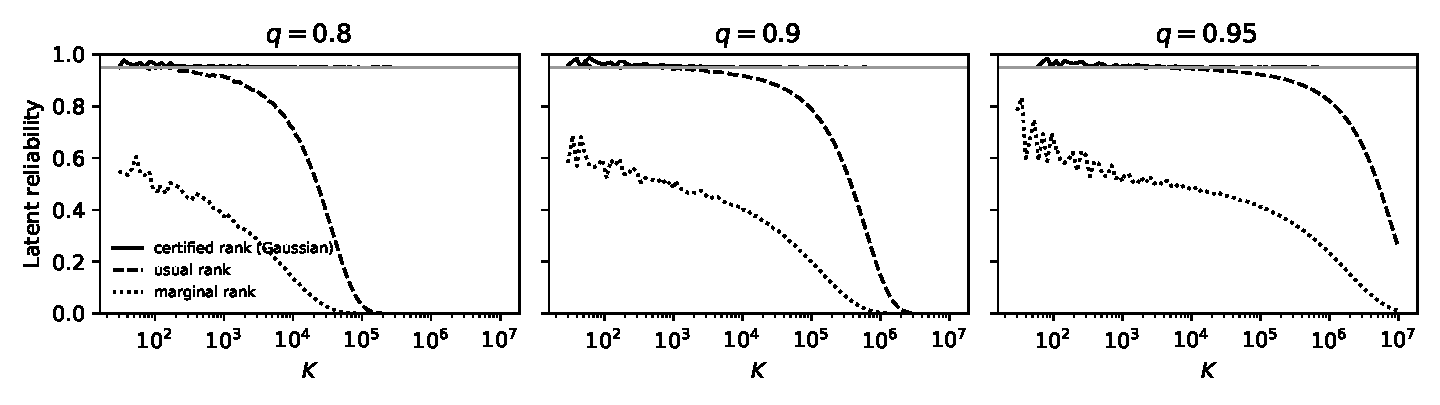
\includegraphics[width=\textwidth]{fig_reliability_q.pdf}
\caption{Exact latent reliability at the extremal law for Gaussian noise, $q = 0.8$, $0.9$ and $0.95$, $\delta = 0.05$: the usual rank loses the guarantee as $K$ grows; the rank of Theorem~\ref{thm:rank} keeps it and tends to $0.95$.}
\label{fig:reliability}
\end{figure}

\begin{table}[htbp]
\renewcommand{\baselinestretch}{1}
\caption{Exact latent reliability at the extremal law for Gaussian noise: rank $k$ and reliability for the usual rank and the rank of Theorem~\ref{thm:rank}}
\label{tab:reliability}
\centering
\fontsize{9}{11pt}\selectfont
\begin{tabular}{ccccccc}
\toprule
& & \multicolumn{2}{c}{usual rank} & \multicolumn{2}{c}{Theorem~\ref{thm:rank}} & marginal \\
$q$ & $K$ & $k$ & reliability & $k$ & reliability & reliability \\
\midrule
$0.8$ & $10^3$ & 822 & 0.915 & 826 & 0.955 & 0.375 \\
 & $10^4$ & 8067 & 0.713 & 8110 & 0.951 & 0.136 \\
 & $10^5$ & 80209 & 0.032 & 80648 & 0.950 & 0.000 \\
$0.9$ & $10^3$ & 916 & 0.943 & 917 & 0.954 & 0.482 \\
 & $10^4$ & 9050 & 0.918 & 9058 & 0.952 & 0.399 \\
 & $10^6$ & 900494 & 0.150 & 901296 & 0.950 & 0.004 \\
$0.95$ & $10^4$ & 9537 & 0.947 & 9538 & 0.952 & 0.477 \\
 & $10^6$ & 950359 & 0.820 & 950518 & 0.950 & 0.233 \\
\bottomrule
\end{tabular}
\end{table}

At $q = 0.8$ the usual rank's reliability falls below $0.9$ at $K \approx 1.4 \times 10^3$ and below $0.5$ at $K \approx 2.5 \times 10^4$; raising the rank from $822$ to $826$ at $K = 10^3$ restores it. The reliability of the usual rank is the share of calibration samples whose interval attains latent coverage $q$; its latent coverage itself is close to $q$, $0.79534$ in the limit at $q = 0.8$. A small coverage shortfall thus destroys the guarantee. The rank of Theorem~\ref{thm:rank} stays above $0.95$ and tends to it, which shows numerically that it cannot be lowered.

Mixed noise laws do not remove the failure. With noise laws drawn per unit from the symmetric unimodal class (Gaussian, uniform, Laplace, $t_3$) or the mean-zero log-concave class, and scales equal or heterogeneous, the exact reliability of the class rank was at least $0.9502$ in all $26$ cases, with the minimum at pure extremal noise, as Theorem~\ref{thm:classes} requires. The usual rank at $q = 0.9$ and $K = 10^5$ had reliability from $0.41$ (pure uniform noise) to $0.92$--$0.94$ (diluted or heterogeneous mixtures), and $10^{-4}$ for mean-zero log-concave noise with the centred exponential law. Heterogeneous scales dilute the excess over $q$, from $0.0018$ to $0.00022$ for uniform noise at $q = 0.9$, because one scale cannot put every unit at its worst; they delay the failure but do not remove it (Supplementary \S~\ref{S-sec:s-mixed}).

\subsection{The cost with the same information}\label{sec:cost}

No rule in this comparison is told the noise law within its class or the variances. Six standardized latent laws were used: normal, Laplace, centred gamma with shape $2$, truncated exponential, a bimodal bi-log-concave mixture that is not log-concave, and $t_3$, which lies outside $\B$, as a control. Eight noise designs, with heterogeneous variances $D_i = 0.577 L_i/E(L_i)$ for $L_i$ lognormal with log-scale $0.7$, comprise five single laws (Gaussian, uniform, Laplace, $t_3$, centred exponential) and laws drawn per unit within the symmetric unimodal class, within the mean-zero log-concave class with both signs of the centred exponential, and across the two classes. Latent coverage given each of $2000$ data sets per setting is exact.

\begin{table}[htbp]
\renewcommand{\baselinestretch}{1}
\caption{Rules with the same information at $K = 1000$: rank and width relative to the usual rank and to the rule for the same noise class without a latent shape assumption, ranges over the settings a rule covers (medians in parentheses)}
\label{tab:sameinfo}
\centering
\fontsize{9}{11pt}\selectfont
\resizebox{\textwidth}{!}{%
\begin{tabular}{lcccccc}
\toprule
& \multicolumn{3}{c}{$q = 0.8$} & \multicolumn{3}{c}{$q = 0.9$} \\
rule & $k$ & above usual (\%) & below no shape (\%) & $k$ & above usual (\%) & below no shape (\%) \\
\midrule
usual & 822 & 0 & -- & 916 & 0 & -- \\
Gaussian & 826 & 0.9--1.2 & 20--26 (24) & 917 & 0.3--0.4 & 16--21 (21) \\
symmetric unimodal & 829 & 1.5--2.2 & 19--28 (24) & 918 & 0.6--1.0 & 15--24 (20) \\
mean-zero log-concave & -- & -- & -- & 922 & 1.8--2.9 & 19--33 (26) \\
no shape, median-zero & 916 & 25--42 & -- & 962 & 18--36 & -- \\
no shape, log-concave & 941 & 36--63 & -- & 974 & 25--54 & -- \\
\bottomrule
\end{tabular}}
\par\smallskip
\parbox{\textwidth}{\fontsize{8}{10pt}\selectfont The log-concave level is certified only at $q = 0.9$. A rule covers a setting when the noise is in its class. The Gaussian and symmetric unimodal rules are compared with the median-zero rule, the log-concave rule with the log-concave one.}
\end{table}

Table~\ref{tab:sameinfo} gives the cost. Every rule had reliability at least $0.998$ in every setting, covered or not, and so did the usual rank: these laws are far from the extremal one, so they measure the cost of the guarantee, not its need. The cost over the usual rank is at most $3\%$ of width at $K = 1000$, and nothing at $K = 110$, where the bi-log-concave ranks equal the usual rank; the saving over the rules without a shape assumption is $15$--$33\%$. At $q = 0.95$ the bi-log-concave ranks equal the usual rank at both $K$, and at $K = 1000$ they save $12$--$23\%$ over the rules without a shape assumption. At $K = 110$ and $q = 0.95$ the rules without a shape assumption have no valid rank at all, while the bi-log-concave rules give $k = 109$: at small $K$ and high $q$, the shape assumption decides whether a valid interval exists. The bimodal law and the mixed designs behaved like the log-concave laws and the single noise laws.

\subsection{Comparison with existing methods}\label{sec:competitors}

Methods that use more information were compared on the same latent laws at $q = 0.9$, with $300$ data sets at $K = 110$ and $200$ at $K = 1000$, and three noise scenarios with the same variances: Gaussian, where the Gaussian forward model of the competitors holds; Laplace; and laws drawn per unit from the symmetric unimodal class. Each rule is judged against its own target: marginal rules by mean latent coverage at least $q$, rules with a high-probability guarantee by reliability at least $1 - \delta$. Table~\ref{tab:competitors} summarizes.

\begin{table}[htbp]
\renewcommand{\baselinestretch}{1}
\caption{Comparison with existing methods at $q = 0.9$: information used, target, whether the target was met over the bi-log-concave latent laws and three noise scenarios, and width relative to the usual rank}
\label{tab:competitors}
\centering
\fontsize{9}{11pt}\selectfont
\resizebox{\textwidth}{!}{%
\begin{tabular}{lllccc}
\toprule
rule & information & target & target met & \multicolumn{2}{c}{width vs usual (\%)} \\
& & & & $K = 110$ & $K = 1000$ \\
\midrule
Theorem~\ref{thm:rank}, Gaussian & none & reliability & yes, $1.000$ & $0$ & $0.3$--$0.5$ \\
Theorem~\ref{thm:rank}, symm.\ unimodal & none & reliability & yes, $1.000$ & $0$ & $0.6$--$0.9$ \\
LatentCP & known $D_i$ & marginal & yes, $\ge 0.970$ & $4$--$7$ & $14$--$21$ \\
LatentCP, tuned & known $D_i$ & marginal & yes, $\ge 0.972$ & $4$--$19$ & $11$--$25$ \\
Markov rule & known $D_i$ & reliability & yes, $1.000$ & $19$--$25$ & $20$--$26$ \\
Fay--Herriot tolerance & known $D_i$ & reliability & no, down to $0.900$ & $-24$ to $-15$ & $-20$ to $-16$ \\
HetLDC & known $D_i$ & reliability & yes, $\ge 0.983$ & about $-10$ & -- \\
known lower bound & known $\min D_i$ & reliability & yes, $1.000$ & $-1.3$ & $0.3$--$0.5$ \\
deconvolution & known $D_i$ & nominal coverage & no, $0.87$--$0.92$ & $-41$ to $-30$ & $-32$ to $-19$ \\
\bottomrule
\end{tabular}}
\par\smallskip
\parbox{\textwidth}{\fontsize{8}{10pt}\selectfont Reliability: share of data sets with latent coverage at least $0.9$; marginal: mean latent coverage. Fay--Herriot met its target for normal latent laws with Gaussian noise; the shortfalls are for the Laplace latent law and for normal latent laws with non-Gaussian noise. HetLDC was run at $K = 110$ under Gaussian noise only. Deconvolution: our implementation of Algorithm~1 of \citet{cohen2025} with bin width $0.2$; with bin width $0.01$ its mean coverage was $0.28$ at $K = 110$. The $t_3$ control is excluded from the widths; with it, the rule of Theorem~\ref{thm:rank} kept reliability $1.000$.}
\end{table}

Three findings stand out. First, the rank of Theorem~\ref{thm:rank}, which uses no noise information, met its target in every setting and was no wider than LatentCP, which is given the variances: LatentCP met its own marginal target throughout, also under Laplace and mixed noise where its Gaussian forward model is wrong, but was $4$--$7\%$ wider at $K = 110$ and $14$--$21\%$ wider at $K = 1000$. This is not a failure of LatentCP, whose target is marginal; it shows that the information it uses does not translate into shorter intervals here. Second, the rules that were shorter use more: HetLDC needs the variances, Gaussian noise and a log-concave latent law, and was about $10\%$ shorter; the Fay--Herriot interval relies on the normal model and lost its high-probability guarantee outside it. Third, the deconvolution threshold, without a finite-sample guarantee, fell below the nominal coverage on average; this may partly reflect tuning, since it depends on the bin width.

%=============================================================================================
\section{Application: school districts}\label{sec:application}

The California Academic Performance Index data \citep{lumley2004} give the 2000 index of every school; districts with at least five schools form the population. Each of $480$ replications, $120$ in each of four conditions, splits the districts into $110$ training, $110$ calibration and the remaining evaluation districts, samples $n = 2$ or $3$ schools per training and calibration district without replacement, fits a ridge predictor on the training schools, using socio-demographic covariates with or without the 1999 index, and centres each district at the population mean of the predictor. The calibration score is the sample-mean residual of a district; its design variance, estimated from $n$ schools, is very noisy. The target of an evaluation district is its true mean residual, and coverage is the share of evaluation districts covered.

At $K = 110$ every class rank of Theorem~\ref{thm:rank} equals the usual rank, $k = 105$, so the intervals coincide with the usual noisy threshold. The point of the application is that this interval now carries a latent guarantee and needs no variance estimates. It covered at least $90\%$ of the evaluation districts in all $480$ replications. It was $19$--$26\%$ wider than the Fay--Herriot tolerance interval, which plugs in the estimated variances and covered fewer than $90\%$ of the districts in up to $9\%$ of the replications of a condition. LatentCP, applied by drawing the unknown variance of a new district from the calibration estimates, covered at least $90\%$ throughout and was $5$--$6\%$ wider than the rank's interval; the Markov rule with plugged-in variances was $12$--$16\%$ wider. The noise class and the latent ordering condition cannot be confirmed from these data (Supplementary \S~\ref{S-sec:s-app}).

%=============================================================================================
\section{Discussion}\label{sec:discussion}

The guarantees hold with probability $1 - \delta$ over calibration samples: on that event, the latent coverage of the new unit, given the calibration data, is at least $q$. They allow noise laws and scales that differ between units within a specified class, independent of the latent residuals, and latent laws that differ between units under the quantile ordering of Corollary~\ref{cor:hetero}. The ordering is the assumption that matters most and is hardest to check; Corollary~\ref{cor:hetero} shows that it cannot be replaced by a shape assumption on each unit. If the new residual is shifted by at most $\rho$ latent standard deviations and the latent law is log-concave, the latent coverage can fall by at most $\rho$, and by $q\rho + O(\rho^2)$ for some laws (Supplementary Proposition~\ref{S-prop:shift}).

Bi-log-concavity cannot be checked on the latent scale, but convolution with log-concave noise preserves it: with a common log-concave noise law, a confidence band for the signed noisy residuals that contains no bi-log-concave distribution function \citep{dumbgen2017} rules it out, though not conversely.

Two questions remain open. For mean-zero log-concave noise the two-sided level is known only within $(0.90517, 0.906]$ at $q = 0.9$, and that the centred exponential law is extremal is supported by certified computation but not proved; the scheme of Theorem~\ref{thm:gauss}, a first-order condition through a Mills ratio of the noise and an envelope derivative through a tilted distribution function, may extend to single log-concave noise laws, but the supremum over the class is a harder problem. Whether bi-log-concavity is necessary for a nontrivial transfer, or some weaker condition excluding a layer of mass at the threshold suffices, is also open.

%=============================================================================================
\section*{Supplementary Material}

The Supplementary Material contains the proofs of all results, including the full proof of Theorem~\ref{thm:gauss} and the comparison lemma for sums of Bernoulli variables; the reduction and certificates for the known-variance results; certificates in ball arithmetic; further simulations, including full tables of \S\S~\ref{sec:need}--\ref{sec:competitors} and the heterogeneous-latent study; details of the application; and a map from every number to the code that produces it. Code is at \texttt{https://github.com/kunhailP/latent-coverage-noisy-calibration}.

\par

\bibhang=1.7pc
\bibsep=2pt
\fontsize{9}{14pt plus.8pt minus .6pt}\selectfont
\renewcommand\bibname{\large \bf References}
\expandafter\ifx\csname natexlab\endcsname\relax\def\natexlab#1{#1}\fi
\expandafter\ifx\csname url\endcsname\relax\def\url#1{\texttt{#1}}\fi
\expandafter\ifx\csname urlprefix\endcsname\relax\def\urlprefix{URL}\fi

\bibliographystyle{chicago}
\bibliography{refs}

\vskip .65cm
\noindent
Kun Woo Park, Department of Political Science and International Relations, Kookmin University, 77 Jeongneung-ro, Seongbuk-gu, Seoul 02707, Republic of Korea
\vskip 2pt
\noindent
E-mail: pkw6094@kookmin.ac.kr

\end{document}
